\section{Lifecycle}

\subsection*{Downloading a Block}

As showin in Figure~\ref{fig:req-life}, a block is downloaded using the following steps:

\begin{enumerate}
  \item The Data Manager component of the backend will choose the enxt block of data to queue and send this over a channel to the Networking component.
  \item The Networking component will attempt to find this block of data from other peers in the network. This gives two scenarios: \begin{enumerate}
    \item \textbf{The block is found} (Proceed to step 3.)
    \item \textbf{The block is not found} \begin{enumerate}
      \item Push the request to a queue of deferred requests.
      \item When we connect to a new peer or a change occurs in one of our peers library, requeue the deferred requests (Go back to Step 2.)
    \end{enumerate}
  \end{enumerate}
  \item The block of data is requested from the peer.
  \item Once received, the block of data will be verified using its hash and inserted into the correct position in the output file.
\end{enumerate}

\begin{figure}[ht]
  \centering
  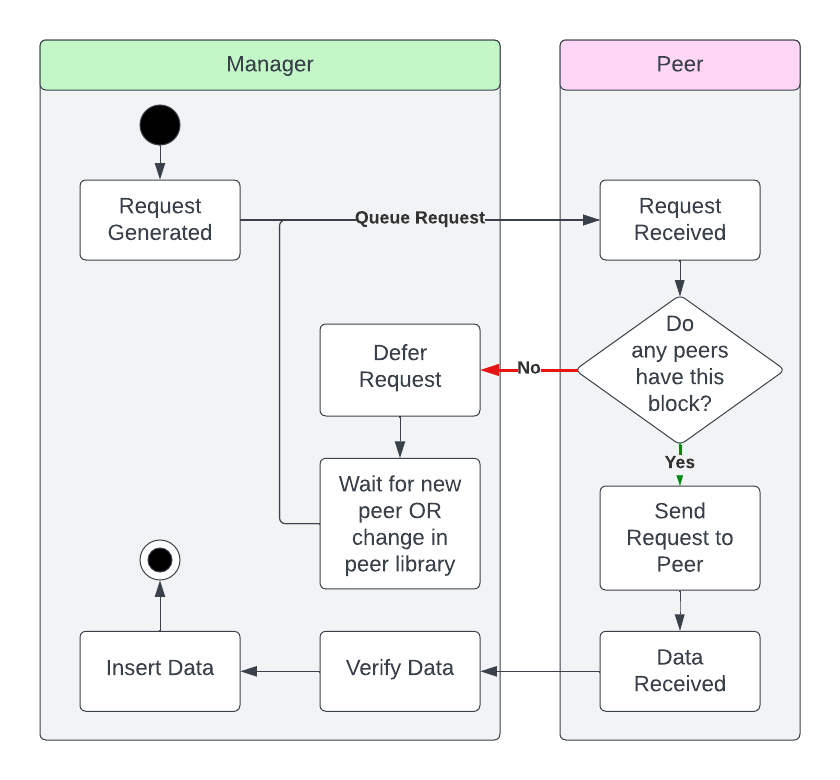
\includegraphics[width=.75\textwidth]{assets/images/diagrams/request-lifecycle.png}
  \caption{The lifecycle of a request for a block of data}
  \label{fig:req-life}
\end{figure}